\chapter{ОЦІНКА ОБЧИСЛЮВАЛЬНОЇ РОБОТИ ЗАСТОСУВАННЯ ПРОГРАМНОГО МОДУЛЮ ПРИ ВИКОНАННІ ТИПОВИХ ЗАВДАННЬ ДОСЛІДЖЕННЯ ПОТЕНЦІЙНО-НЕБЕЗПЕЧНИХ ДЕФЕКТІВ ЦІЛЬОВИХ ПРОГРАМ}
\label{4section::doc}\label{4section:id1}

Програмним продуктом, який буде досліджено, буде один із модулів веб-серверу {\it nginx}, а саме, {\it TFS}.

\begin{figure}[h]
    \centering
    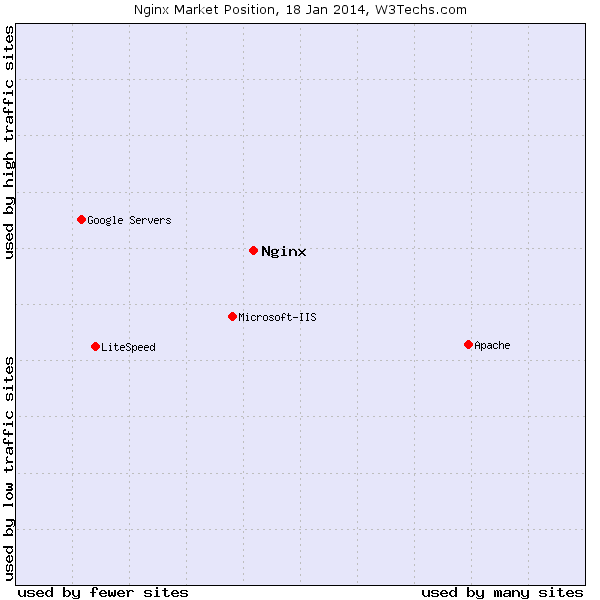
\includegraphics[width=12cm]{ws-nginx.png}
    \caption{статистика використання {\it nginx} за 18 січня 2014 року згідно {\it W3Techs} }
    \label{fig:nginx_statics_image}
\end{figure}

{\it nginx} — це вільний веб-сервер і проксі-сервер. Є версії для сімейства {\it Unix}-подібних операційних систем {\it(FreeBSD, GNU/Linux, Solaris, Mac OS X)} та {\it Microsoft Windows}.

Згідно з квітневим 2012 року звітом компанії {\it Netcraft nginx} використовується на 12.76\% всіх активних сайтів і на 10.09\% з мільйона найвідвідуваніших сайтів у світі. За рік до того {\it nginx} використовувався на 8.68\% всіх активних сайтів і 6.52\% популярних сайтів. За рік {\it nginx} переступив десятивідсоткову межу і витіснив {\it IIS} на третє місце в рейтингу популярності активних сайтів. Звіт налічує близько 23.4 млн хостів під управлінням {\it nginx}.
За даними {\it W3Techs} на 18 січня 2014 11\% з мільйона найвідвідуваніших сайтів у світі використовують {\it nginx}, тоді як у квітні 2011 року цей показник становив 6.8\%. У Росії {\it nginx} використовується на 58.2\% найбільш відвідуваних сайтів (рік тому — 46.9\%) (Рис.\,\ref{fig:nginx_statics_image}).

{\it TFS} це розподілена файлова система, розроблена {\it Taobao}.
Метою розподіленої файлової системи з високою доступністю, високою продуктивністю і низькою вартістю, {\it TFS}-це {\it linux}-файлова система, яка забезпечує високу надійність і паралельного доступу за рахунок дублювання, копіювання і технології балансування навантаження. {\it TFS}, в основному, призначений для невеликих файлів (менше 1 Мб. Він приймає плоску структуру замість традиційної структури каталогів. {\it TFS} буде генерувати 18 байт довжини файлу після збереження даних для завантаження файлів. Користувачі можуть отримувати доступ до своїх даних з унікальним ім'ям.


\section{Опис випробування (натурного)}
\label{4section:id2}
% localhost:8080/serve/fSdR1er1QyQcOQOBf_xNyg%3D%3D

Ефективність програмного забезпечення — характеристика програмного забезпечення, ступінь відповідності ПМ до вимог. При цьому вимоги можуть трактуватись по-різному, що породжує декілька незалежних визначень терміну. Частіше за все, використовують визначення {\it ISO 9001}, згідно з яким якість – це \dq ступінь відповідності наявних характеристик вимогам\dq.

Фактори ефективності  — це нефункціональні вимоги до ПМ, що відносяться до, наприклад, надійності та продуктивності програм.

Для оцінки ефективності розробленого програмного забезпечення використано такі основні фактори:
\begin{itemize}
\item Зрозумілість - Призначення ПМ повинно бути зрозумілим з самої програми та документації.
\item Повнота - Всі необхідні частини програми повинні бути представлені та реалізовані.
\item Стислість - Відсутність надлишкової інформації та такої, що дублюється.
\item Можливість портування - Легкість в адаптації програми до інших умов: архітектури, платформи, операційної системи тощо.
\item Узгодженість - Вся документація та код повинні виконуватися за єдиними угодами, використовувати єдині формати та позначення
\item Зручність використання - Простота та зручність використання програми. Ця вимога відноситься в першу чергу до інтерфейсу користувача.
\item Надійність - Відсутність відмов та збоїв у роботі програми, а також простота виправлення помилок.
\item Ефективність - Наскільки раціонально програма відноситься до ресурсів (пам’ять, процесор) при виконанні своїх задач.
\item Безпечність.
\end{itemize}

\subsection{Зрозумілість}\label{mark_understand}
Призначення розробленого програмного модулю – полегшити роботу при аналізі програмних продуктів з метою використання їх вразливостей, та забезпечити досягнення мети у повному обсязі. Призначення являється зрозумілим, а документація користувача надає вичерпні відповіді щодо роботи програмного модулю, завдяки чому суть його призначення можна вважати доступним.

\subsection{Повнота}\label{mark_fully}
Програмний продукт являє собою першу версію програмного додатка для аналізу вихідних текстів програмних продуктів на предмет наявності доступних у використанні потенційно-небезпечних вразливостей. Усі функції, покладені на дане програмне забезпечення реалізовані у повному обсязі згідно до зазначених заздалегідь вимог, та працюють коректно.

\subsection{Стислість}\label{mark_compact}
Програмний продукт був неодноразово перевірений і протестований на наявність зайвих та дубльованих процедур та функцій. У результаті перевірок надлишкової та дубльованої інформації виявлено не було.

\subsection{Можливість портування}\label{mark_portability}
Даний програмний продукт був реалізований за допомогою мови програмування {\it Python}, що надає змогу користувачу  застосовувати його на більшості поширених операційних систем, на які портовано інтерпретатор {\it Python}.

\subsection{Узгодженість}\label{mark_correct}
Призначення розробленого програмного модулю – полегшити роботу при аналізі програмних продуктів з метою використання їх вразливостей, та забезпечити досягнення мети у повному обсязі. Призначення являється зрозумілим, а документація користувача надає вичерпні відповіді щодо роботи програмного модулю, завдяки чому суть його призначення можна вважати доступним.

\subsection{Зручність використання}\label{mark_usability}
Питання зручності використання створеного програмного продукту задовольняється наявністю легкого в експлуатації інтерфейсу користувача, наявністю максимально зрозумілої довідки користувача, а також легкості у супроводженні з точки зору користувача-програміста.
Однією з висунутих заздалегідь вимог до програмного продукту була відкритість коду. Ця вимога реалізована, і надає можливість у будь-який час за потреби внести власні зміни до версії програмного продукту.
Інтерфейс користувача реалізований таким чином, щоб максимально забезпечити зручність у застосуванні. Він є інтуїтивно зрозумілим для будь-якого користувача з базовими знаннями по роботі з ЕОМ.

\subsection{Безпечність}\label{mark_security}
Обробка інформації під час застосування здійснюється на серверній частині програмного продукту, а не на сторонньому сервері. Це виключає можливість потрапляння інформації стороннім особам, і являється суттєвим внеском у питання безпеки.

Оцінка отриманих результатів.

В якості показника для цього виду оцінки використовують:
\begin{enumerate}
\item Скорочення часу вирішення задачі при використання ЕОМ (T,r) обраховується за формулою:

\begin{equation}\label{f:T}
  T = \cfrac{Tp-Ta}N
\end{equation}

де:

Тр – час вирішення задачі без ЕОМ;

Та – час вирішення задачі на ЕОМ;

N – частота вирішення задачі.

\item Відповідно до формули \eqref{f:T}  Тр обраховується за формулою:

\begin{equation}\label{f:Tp}
  Tp = \textup{Тпр}+\textup{Трр}+\textup{Тор}
\end{equation}

де:

Тпр – час збору і підготовки вихідних даних для вирішення задачі вручну (40 хв.);

Трр – час вирішення задачі  (15 хв);

Тор – час на оформлення результатів вирішення (5 хв).

В нашому випадку Тр=60 хв.

\item Відповідно до формули \eqref{f:T} Та обраховується за формулою:

\begin{equation}\label{f:Ta}
  Ta = \textup{Тпа}+\textup{Тра}+\textup{Тоа}
\end{equation}

де:

Тпа – час збору інформації для вводу в ЕОМ (5 с);

Тра – час вирішення задачі на ЕОМ (2 с);

Тоа – час обробки і оформлення результату (0.3 с).

В нашому випадку Та=7,5 с.

\end{enumerate}

Коефіцієнт відносної економії часу при вирішенні задачі на ЕОМ (КОСТ,\%) обраховується за формулою:

\begin{equation}
  KOCT = \cfrac{Tp-Ta}{Tp}100\% = \cfrac{T}{N*Tp}100\%
\end{equation}

В нашому випадку КОСТ=99.78\%.
Показник ефективності по часу вирішення зростає зі збільшенням об’єму інформації, яка обробляється та частоти вирішення задачі.

\subsection{Надійність}\label{mark_relayeble}
Програмний продукт був повність протестований на наявність помилок та збоїв при роботі. Після ряду тестів та пробного практичного застосування було відлагоджено усі наявні недоліки. Окрім цього було розроблено ряд {\it unit}-тестів, що дозволило частково автоматизувати процес тестування та звільнитись від більшості ручних операцій.

\subsection{Ефективність}\label{mark_afford}
Задля оцінки ефективності було проведено наступний експеримент: на вхід аналізатора було подано файл вихідного коду програми, який містив вразливості переповнення буфера різних типів : переповнення стеку, кучі, переповнення керуючих змінних. На виході було отримано перелік потенційно вразливих елементів проекту.

\pagebreak

\section{Порівняльний аналіз результатів}
\label{4section:id3}
Після завантаження досліджуваного модулю на сервер, було проведено аналіз і отримано наступні результати:

\npdecimalsign{.}
\nprounddigits{2}
\begin{center}
  \begin{tabular}{
  |l|c|c|c|n{3}{2}|c|n{2}{2}|n{2}{2}|
  }
  \hline 
  назва файлу &  
  SLOC & 
  \parbox[t]{1cm}{V} & 
  \parbox[t]{1cm}{Z(G)} & 
  Rup & 
  vulns & 
  P & 
  p\\
  
  \hline rc\_server\_message.c & 818 & 2852.0 & 2.61 & 168.7459 & 1 & 0.154427348878 & 0.5\\
  \hline common.c & 834 & 2376.0 & 1.29 & 214.2913 & 1 & 0.11634502399 & 0.5\\
  \hline json.c & 345 & 1104.0 & 2.08 & 67.5407 & 1 & 0.127250594203 & 0.5\\
  \hline module.c & 1246 & 3422.0 & 1.7 & 267.278 & 1 & 0.132779836353 & 0.5\\
  \hline raw\_fsname.c & 180 & 1083.0 & 1.86 & 79.427 & 1 & 0.136412022161 & 0.5\\
  \hline local\_block\_cache.c & 443 & 1506.0 & 2.26 & 83.8424 & 1 & 0.125819272244 & 0.5\\
  \hline peer\_connection.c & 464 & 1589.0 & 3.67 & 96.2391 & 1 & 0.222276587162 & 0.5\\
  \hline timers.c & 185 & 522.0 & 1.87 & 41.8555 & 1 & 0.149942116858 & 0.5\\
  \hline block\_cache.c & 163 & 464.0 & 1.32 & 32.5766 & 1 & 0.0926748103448 & 0.5\\
  \hline common.h & 286 & 580.0 & 1.56 & 119.025 & 1 & 0.320136206897 & 0.5\\
  \hline duplicate.c & 546 & 1597.0 & 1.78 & 106.006 & 1 & 0.118153212273 & 0.5\\
  \hline name\_server\_message.c & 873 & 2971.0 & 2.87 & 166.1117 & 1 & 0.160464684955 & 0.5\\
  \hline root\_server\_message.c & 71 & 208.0 & 1.58 & 28.5181 & 1 & 0.216627875 & 0.5\\
  \hline server\_handler.c & 1490 & 4235.0 & 2.69 & 257.1846 & 1 & 0.163359285478 & 0.5\\
  \hline restful.c & 754 & 2370.0 & 3.68 & 102.0978 & 1 & 0.158531605063 & 0.5\\
  \hline connection\_pool.c & 322 & 924.0 & 1.82 & 66.2098 & 1 & 0.130413242424 & 0.5\\
  \hline data\_server\_message.c & 1633 & 5848.0 & 3.12 & 265.8103 & 1 & 0.141813976744 & 0.5\\
  \hline rc\_server\_info.c & 324 & 1032.0 & 1.86 & 73.0801 & 1 & 0.131714133721 & 0.5\\
  \hline tfs.c & 2281 & 7339.0 & 2.46 & 449.199 & 1 & 0.150569497207 & 0.5\\
  \hline meta\_server\_message.c & 829 & 3058.0 & 2.78 & 179.3588 & 1 & 0.163053454545 & 0.5\\
  \hline remote\_block\_cache.c & 484 & 1465.0 & 1.84 & 94.2824 & 1 & 0.118416120137 & 0.5\\
  \hline tair\_helper.c & 187 & 542.0 & 1.33 & 28.2889 & 1 & 0.0694174114391 & 0.5\\
  \hline 
 \end{tabular}
\end{center}
\npnoround

Як видно з таблиці, даний програмний модуль містить ряд помилок, і ймовірність їх використання є середньою - для більш точних даних необхідна більша кількість досліджуваних проектів та експертних оцінок фахівців даної області.

\pagebreak

\section*{Висновки}
\addcontentsline{toc}{section}{Висновки}
Даний програмний комплекс успішно справляється з задачами дослідження та  пошуку потенційно-небезпечних дефектів реакції програм, збереженням та візуалізацією даних аналізу. Він є простим та інтуїтивним в використанні, не потребує глибоких знань та навичок аналізу коду а тому є придатним для швидкого ознайомлення з інтегрованими властивостями досліджуваного програмного продукту. 
